\chapter{Resultados}

Para a execução bem-sucedida do projeto, foi necessário seguir uma metodologia estruturada que envolveu diversas etapas de desenvolvimento interconectadas. Inicialmente, realizou-se uma fase de familiarização com o ecossistema tecnológico da Tuya, incluindo a compreensão da arquitetura da plataforma IoT, suas APIs e protocolos de comunicação. Subsequentemente, foi conduzido um estudo aprofundado dos módulos e componentes envolvidos, abrangendo desde as tecnologias de orquestração de dados (Dagster) até as ferramentas de desenvolvimento de interfaces web (Streamlit). A análise detalhada dos requisitos funcionais e não-funcionais permitiu estabelecer uma base sólida para o desenvolvimento, seguida pela elaboração de documentação técnica abrangente que descreveu todo o processo de implementação, a arquitetura do sistema e o relacionamento entre os diversos módulos. Finalmente, as fases de implementação e testes foram executadas de forma iterativa, garantindo a validação contínua das funcionalidades desenvolvidas e a conformidade com os requisitos estabelecidos.

\section{Atividades do Projeto}
\label{sec:atividades_projeto}
O desenvolvimento do projeto envolveu uma série de atividades interligadas, desde a concepção inicial até a implementação e validação. As principais fases incluíram a pesquisa e análise de tecnologias existentes, o projeto da arquitetura do sistema, a implementação do pipeline de dados e da interface de usuário, e a validação em ambiente real.

\section {Requisitos do Sistema}
\label{sec:requisitos_sistema}
Os requisitos do sistema foram definidos para garantir que a solução proposta atendesse às necessidades de monitoramento e controle de dispositivos inteligentes, bem como à análise de consumo de energia. Estes requisitos abrangeram desde a capacidade de integração com a API da Tuya até a apresentação intuitiva dos dados e a funcionalidade de agendamento de cenas.

\section{Desenvolvimento e Implementação}
\label{sec:desenvolvimento_implementacao}

A implementação do sistema compreendeu duas frentes principais: o pipeline de dados orquestrado pelo Dagster e a aplicação de interface do usuário desenvolvida com Streamlit.

\subsection{Pipeline de Dados com Dagster}
\label{sec:dagster_pipeline}
O pipeline de dados foi projetado para coletar, processar e armazenar informações de consumo de energia dos dispositivos Tuya de forma automatizada e robusta. A orquestração desse processo foi realizada utilizando o framework Dagster, que permitiu a definição de ativos (assets), trabalhos (jobs) e agendamentos (schedules) para gerenciar o fluxo de dados.

O pipeline é composto por dois ativos principais:
\begin{itemize}
    \item \texttt{raw\_tuya\_logs}: Este ativo é responsável pela ingestão dos dados brutos diretamente da API da Tuya. Ele utiliza a biblioteca \texttt{tuya-connector-python} para interagir com a nuvem da Tuya, coletando logs de eventos e informações de consumo. Os dados brutos são então enriquecidos com metadados como \texttt{device\_id} e informações de ingestão, e salvos como arquivos JSON particionados por ID do dispositivo e data no diretório \texttt{app/data/raw/}.
    \item \texttt{staging\_tuya\_logs}: Dependente do ativo \texttt{raw\_tuya\_logs}, este ativo realiza o processamento dos dados brutos para uma camada de \textit{staging}. Ele utiliza o DuckDB, um sistema de gerenciamento de banco de dados analítico em processo, para carregar e transformar os arquivos JSON. O mapeamento de dispositivos (\texttt{app/data/device\_mapping.json}) é carregado com Pandas e registrado como uma visão no DuckDB para enriquecimento dos dados. As transformações incluem a conversão de \texttt{event\_time} para um formato de timestamp legível, adição de \texttt{filename} e junção com \texttt{device\_name}. Os dados processados são então salvos como arquivos Parquet particionados por \texttt{event\_date} no diretório \texttt{app/data/staging/}.
\end{itemize}

O fluxo é encapsulado no trabalho \text{tuya\_processing\_job}, executado de hora em hora pelo agendamento \texttt{hourly\_schedule}.

\begin{figure}[htbp]
    \centering
    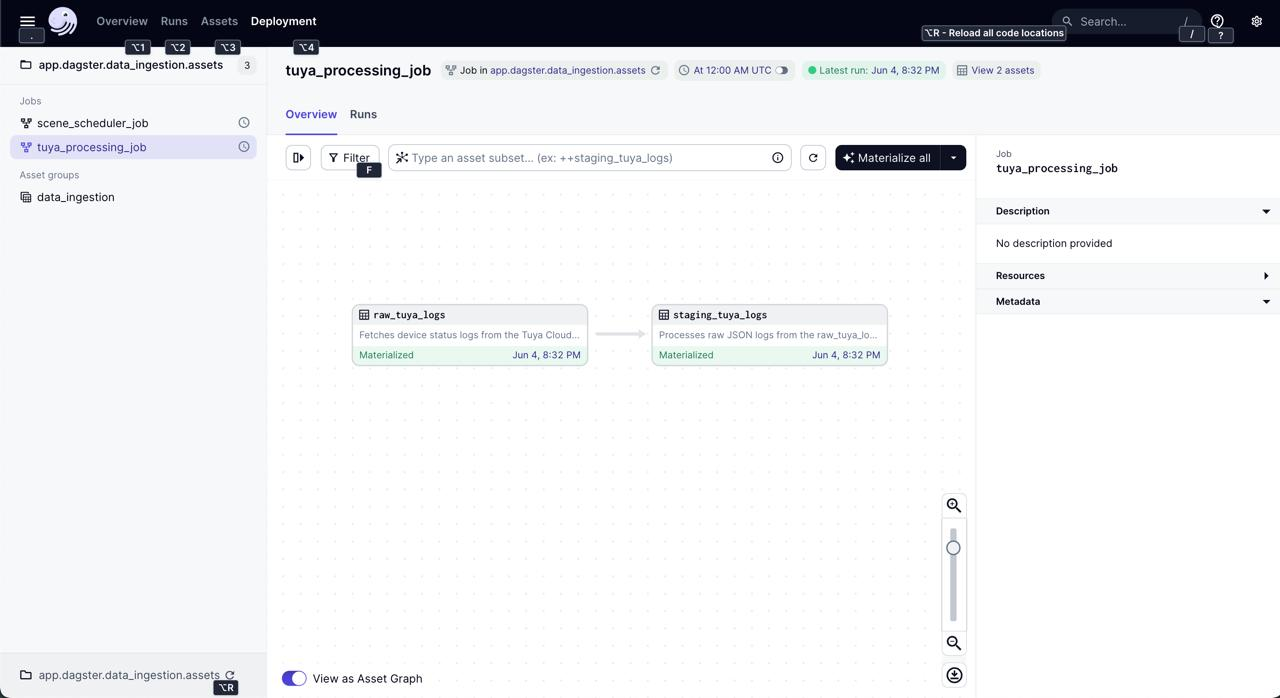
\includegraphics[width=0.8\textwidth]{Resultados/Figuras/dagster_data_pipeline.png.jpeg}
    \caption{Pipeline de Dados com Dagster: ativos \texttt{raw\_tuya\_logs} e \texttt{staging\_tuya\_logs}.}
    \label{fig:dagster_pipeline}
\end{figure}

Além do pipeline de dados, o Dagster também foi utilizado para orquestrar o agendamento de cenas. Um recurso (\texttt{resource}) \texttt{tuya\_api\_resource} foi criado para gerenciar as credenciais da API da Tuya. A operação (\texttt{op}) \texttt{check\_and\_trigger\_scenes\_op} lê as cenas agendadas do arquivo \texttt{scheduled\_scenes.json}, verifica quais cenas estão prontas para serem executadas com base em seus horários e dias de recorrência, e aciona os comandos correspondentes via API da Tuya. Esta operação é encapsulada no trabalho \texttt{scene\_scheduler\_job}, que é executado a cada minuto por meio do agendamento \texttt{scene\_execution\_schedule}.

\begin{figure}[htbp]
    \centering
    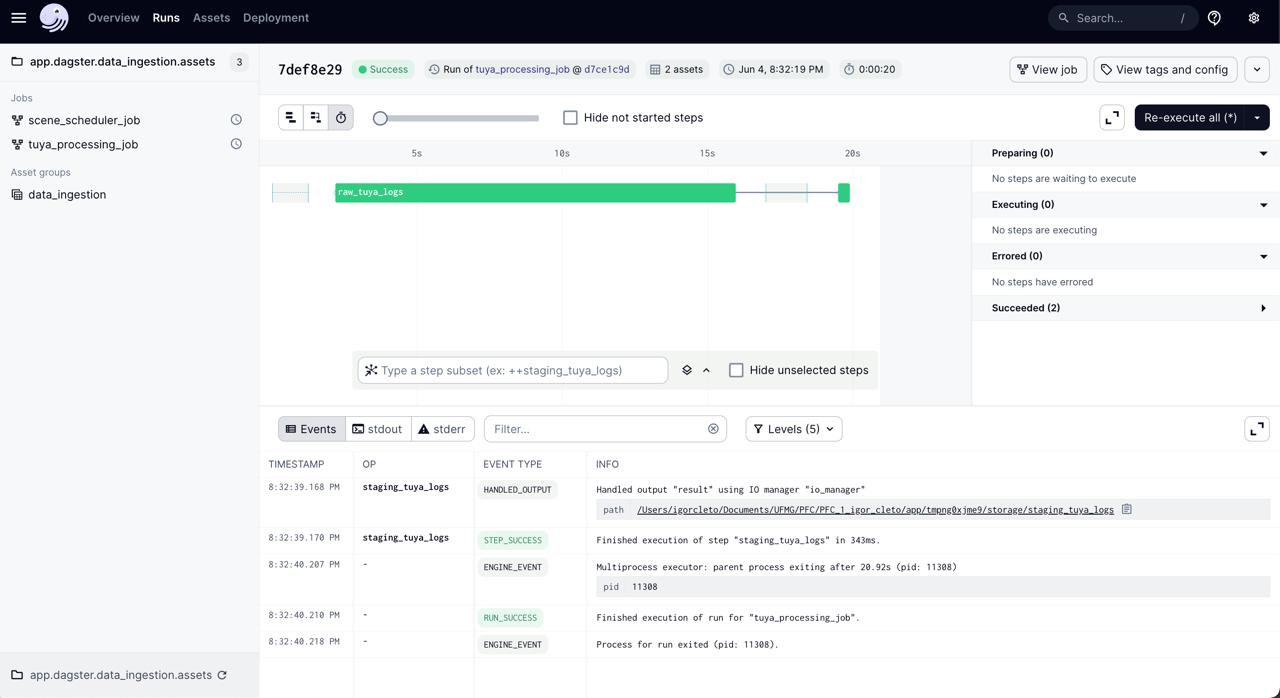
\includegraphics[width=0.8\textwidth]{Resultados/Figuras/dagster_data_pipeline_02.png.jpeg}
    \caption{Trigger de execução de cenas do Pipeline de Dados com Dagster.}
    \label{fig:dagster_data_pipeline_new}
\end{figure}

\begin{figure}[htbp]
    \centering
    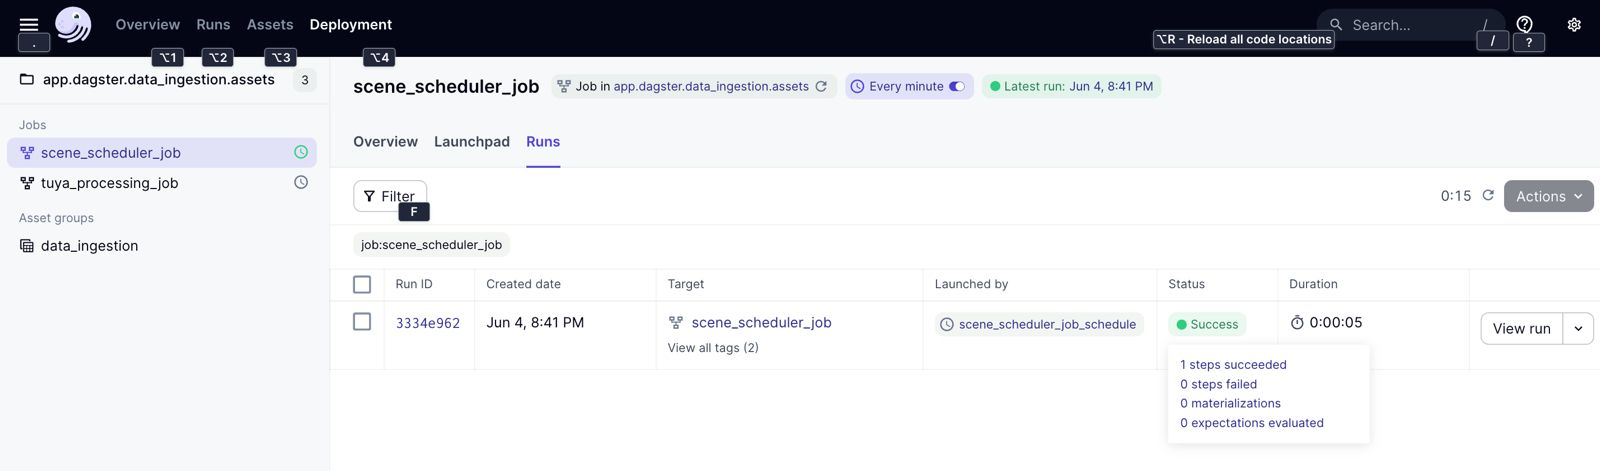
\includegraphics[width=0.8\textwidth]{Resultados/Figuras/dagster_scene_scheduler.png.jpeg}
    \caption{Interface do Dagster exibindo o job de agendamento de cenas (\texttt{scene\_scheduler\_job}) e seu schedule.}
    \label{fig:dagster_scene_scheduler_resultados}
\end{figure}

\subsection{Aplicação de Interface do Usuário com Streamlit}
\label{sec:streamlit_app}
A aplicação web desenvolvida com Streamlit serve como a interface principal para o usuário interagir com o sistema, visualizar dados de consumo de energia e controlar dispositivos. A aplicação foi redesenhada com foco na experiência do usuário doméstico, adotando uma navegação multi-página via barra lateral.

As principais páginas e funcionalidades da aplicação incluem:

\begin{itemize}
    \item Resumo da Casa: Esta página oferece uma visão consolidada do consumo de energia da residência. Apresenta métricas totais de consumo (kWh) para períodos como "Hoje", "Últimos 7 Dias" e "Este Mês". Inclui também uma seção de "Principais Consumidores", que lista os 5 dispositivos com maior consumo de energia, acompanhada de um gráfico de barras, e uma análise consolidada de potência.
    \begin{figure}[htbp]
        \centering
        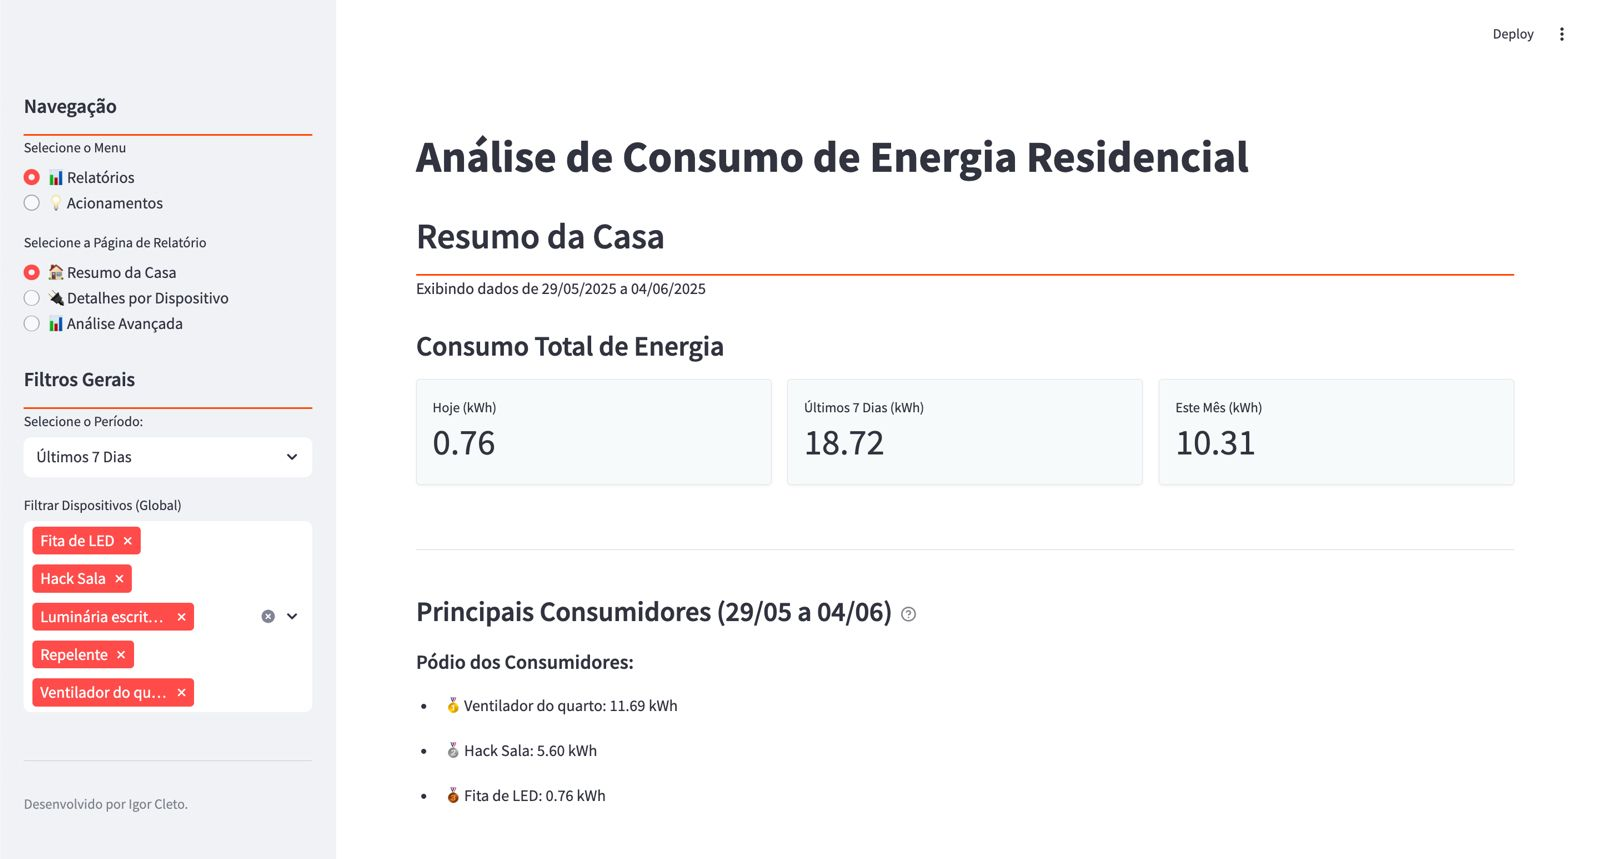
\includegraphics[width=0.9\textwidth]{Resultados/Figuras/streamlit_resumo_casa.png.jpeg}
        \caption{Página "Resumo da Casa" na Aplicação Streamlit, exibindo métricas de consumo e principais consumidores.}
        \label{fig:streamlit_resumo_casa}
    \end{figure}
\end{itemize}
